
In this section, we present the main algorithm of the compiler, that turns
inference rules into C++ code, and we discuss the key optimizations for
efficient code execution.

\subsection{Constraints}

After an inference rule is compiled, it must respect the \emph{fact constraints}
(facts must exist in the database) and the \emph{join constraints} that can be
represented by variable constraints and/or boolean expressions. For instance,
consider again the second rule of the SSSP program presented in
Fig.~\ref{code:shortest_path_program}:

\begin{Verbatim}[fontsize=\scriptsize,label=example_rule]
shortest(A, D1, P1), D1 <= D2, relax(A, D2, P2)
   -o shortest(A, D1, P1).
\end{Verbatim}

The fact constraints include the facts required to trigger the rule, namely
\texttt{shortest(A, D1, P1)} and \texttt{relax(A, D2, P2)}, and the join
constraints include the expression \texttt{D1 <= D2}.

However, rules may also have other less obvious join constraints such as
variable constraints in the following rule:

\begin{Verbatim}[fontsize=\scriptsize]
new-neighbor-pagerank(A, B, New),
neighbor-pagerank(A, B, Old)
   -o neighbor-pagerank(A, B, New).
\end{Verbatim}

\noindent where variable \texttt{B} must have the same value in both body
facts\footnote{Rule taken from an asynchronous PageRank program.}.

\subsection{Iterators}

The data structures for facts presented in Section~\ref{sec:data_structures}
support the \emph{iterator} pattern. For linked lists, the iterator goes
through every fact in the list while the hash table iterator can either iterate
through the whole table or iterate through a single bucket. A bucket iterator is
in fact a linked list iterator that starts from a given argument.
For tries, while the default iterator goes through every fact in
the trie, it can be customized with a matching specification in
order to reduce search. A matching specification includes argument
assignments (e.g., argument $i = V$, where $V$ is a concrete value).

Iterators are heavily used in the compiled code. For instance, the second rule
of the SSSP program presented in Fig.~\ref{code:shortest_path_program} is
compiled as follows:

\begin{Verbatim}[numbers=left,fontsize=\scriptsize,xleftmargin=\codemargin]
for(auto it1(list("shortest").begin()); it1 != list("shortest").end(); ) {
   fact *f1(*it1);
   for(auto it2(list("relax").begin()); it2 != list("relax").end(); ) {
      fact *f2(*it2);
      if(f1->get_int(1) <= f2->get_int(1)) { // D1 <= D2
         fact *new_shortest(new fact("shortest"));
         new_shortest->set_int(1, f1->get_int(1));
         new_shortest->set_list(2, f1->get_list(2));

         // new fact was derived
         list("shortest").push_back(new_shortest);

         // deleting facts
         it1 = list("shortest").erase(it1); // remove from list
         it2 = list("relax").erase(it2);
         return;
      }
      ++it2;
   }
   ++it1;
}
\end{Verbatim}


The compilation algorithm iterates through the fact expressions in the body of
the rule and creates nested loops to try all the possible combinations of facts.
For this rule, all pairs of \texttt{shortest} and \texttt{relax} facts must be
matched until the constraint \texttt{D1 <= D2} is true. First, an iterator for
\texttt{shortest} is created that will loop through all \texttt{shortest} facts
in the list. Inside the loop, a nested iterator is created for predicate
\texttt{relax}. This inner loop includes a check for the \texttt{D1 <= D2}
constraint. If the constraint fails, another \texttt{relax} fact is then
attempted by incrementing \texttt{it2}. Likewise, if the current \texttt{f1}
fact fails for all \texttt{f2} facts, then \texttt{it1} is incremented in order
to try the next \texttt{shortest} fact. Otherwise, if the constraint succeeds
then the rule matches and a new \texttt{shortest} fact is derived. Additionally,
the two used linear facts are retracted by erasing the iterators from the linked
lists.  Note that after the rule is derived, the code must return since there is
a higher priority rule that may be triggered with the new \texttt{shortest} fact
(see Fig.~\ref{fig:shortest_path_program}). This enforces the priority semantics
of the language.
    

\begin{figure}
\begin{algorithm}[H]
 \KwData{Rule R1, Rules}
 \KwResult{Compiled Code}
 $FactExprs \longleftarrow FactExprsFromRule(R1)$\;
 $Constraints \longleftarrow ConstraintsFromRule(R1)$\;
 $Code \longleftarrow CreateFunctionForRule()$\;
 $Iterators \longleftarrow []$\;
 $CompiledFacts = []$\;
 \While{$FactExprs$ not empty}{
  $Fact \longleftarrow RemoveBestFactExpr(FactExprs)$\;
  $CompiledFacts.push(Fact)$\;
  $Iterator \longleftarrow Code.InsertIterator(Fact)$\;
  $Iterators.push(Iterator)$\;
  \tcc{Select constraints that are covered by CompiledFacts.}
  $NextConstraints \longleftarrow RemoveConstraints(Constraints, CompiledFacts)$\;
  $Code.InsertConstraints(NextConstraints)$\;
 }
 $HeadFacts = HeadTemplatesFromRule(R1)$\;
 \While{$HeadFacts$ not empty}{
    $Fact \longleftarrow RemoveFact(HeadFacts)$\;
    $Code.InsertDerivation(Fact)$\;
 }
 \For{$Iterator \in Iterators$}{
    \If{$IsLinear(Iterator)$}{
       $Code.InsertRemove(Iterator)$\;
    }
 }
 \tcc{Enforce rule priorities.}
 \uIf{$FactsDerivedUsedBefore(Head, Program, R1)$}{
    $Code.InsertReturn()$\;
 }
 \Else{
    $Code.InsertGoto(FirstLinear(Iterators))$\;
 }
 \Return{$Code$}
\end{algorithm}
 \caption{Compiling LM rules into C++ code.}
 \label{alg:compile_rule}
\end{figure}

Figure~\ref{alg:compile_rule} presents the algorithm for compiling rules into
C++ code. First we split the body of the rule into fact expressions and
constraints. Fact expressions map directly to iterators while fact constraints
map to \emph{if} expressions. A possible compilation strategy is to first
compile all the fact expressions and then compile the constraints. However, this
may require unneeded database lookups since some constraints may fail early.
Therefore, our compiler introduces constraints as soon as all the variables in
the constraint are all included in the already compiled fact expressions. The
order in which fact expressions are selected for compilation does not interfer
with the correctness of the compiled code, thus our compiler selects the fact
expressions ($RemoveBestFactExpr$) by their potential to activate constraints,
therefore avoiding undesirable database lookups. If two fact expressions have
the same number of new constraints, then the compiler always picks the
persistent fact expression since persistent facts are not deleted.

Derivation of new facts belonging to the local node implies adding the new fact
to the local node data structure. Facts that belong to other nodes are sent
using an appropriate runtime API.

\subsection{Persistence Checking}

Not all linear facts need to be deleted. For instance, in the compiled rule
above, the fact \texttt{shortest(A, D1, P1)} is re-derived in the head. Our
compiler is able to turn linear loops into persistent loops for linear facts
that are retracted and then asserted.  The rule is then compiled as follows:

\begin{Verbatim}[numbers=left,fontsize=\scriptsize,xleftmargin=\codemargin]
for(auto it1(list("shortest").begin()); it1 != list("shortest").end(); ) {
   fact *f1(*it1);
   for(auto it2(list("relax").begin()); it2 != list("relax").end(); ) {
      fact *f2(*it2);
      if(f1->get_int(1) <= f2->get_int(1)) {
         it2 = list("relax").erase(it2);
         goto next;
      }
      ++it2;
next: continue;
   }
   ++it1;
}
\end{Verbatim}

In this new version of the code, only the \texttt{relax} facts are deleted,
while the \texttt{shortest} facts remain untouched. In the SSSP program, each
node has one \texttt{shortest} fact and this compiled code simply filters out
the \texttt{relax} facts with the distances that are equal or greater than the
current best distance. Note that now we have a \emph{goto statement} (line 7)
that is executed when the rule is fired.  In this case, since no new
\texttt{shortest} fact was derived, we can avoid returning to enforce rule
priorities and we can continue to try to fire the rule as many times as
possible.

All the rule combinations are attempted in cases where a rule does not derive
any facts or the facts derived do not appear before the rule, that is, the new
facts are only used in lower priority rules. This is specified in the final
\emph{if statement} in Fig.~\ref{alg:compile_rule}. If the rule does not return,
then we always jump to the first loop that uses linear facts. We must jump to
the first linear loop because we cannot use the next fact from the deepest loop
since we may have constraints between the first linear loop and the deepest loop
that were validated using deleted facts.

\subsection{Updating Facts}

Many inference rules retract and then derive the same predicate but with
different arguments. The compiler recognizes those cases and instead of
retracting the fact from its linked list or hash table, it updates the fact
in-place. As an example, consider the following rule:

\begin{Verbatim}[fontsize=\scriptsize]
new-neighbor-pagerank(A, B, New),
neighbor-pagerank(A, B, Old)
   -o neighbor-pagerank(A, B, New).
\end{Verbatim}

Assuming that \texttt{neighbor-pagerank} is stored in a hash table and indexed
by the second argument, the code for the rule above is as follows:

\begin{Verbatim}[numbers=left,fontsize=\scriptsize,xleftmargin=\codemargin]
for(auto it1(list("new-neighbor-pagerank").begin()); it1 !=
   list("new-neighbor-pagerank").end(); )
{
   fact *f1(*it1);
   // hash table for neighbor-pagerank is indexed by the second argument therefore
   // we search for the bucket using the second argument of new-neighbor-pagerank
   hash_bucket bucket(hash_table("neighbor-pagerank").find(f1->get_node(1));
   for(auto it2(bucket.begin()); it2 != bucket.end(); ) {
      fact *f2(*it2);
      if(f1->get_node(1) == f2->get_node(1)) {
         f2->set_float(2, f1->get_float(2)); // update neighbor-pagerank
         it1 = list("new-neighbor-rank").erase(it1);
         goto next;
      }
      ++it2;
   }
   ++it1;
next: continue;
}
\end{Verbatim}

Note that \texttt{neighbor-pagerank} is updated using \texttt{set\_float}. The
rule also does not return since this is the highest priority rule. If there
was a higher priority rule using \texttt{neighbor-pagerank}, then the code
would have to return since an update fact represents a new fact.

\subsection{Enforcing Linearity}

We have already introduced the \emph{goto} statement as a way to avoid reusing
retracted linear facts. However, this is not enough in order to enforce
linearity of facts. Consider the following inference rule:

\begin{Verbatim}[fontsize=\scriptsize]
add(A, N1), add(A, N2) -o add(A, N1 + N2).
\end{Verbatim}

Using the standard compilation algorithm, two nested loops are created, one for
each \texttt{add} fact. However, notice that there is an implicit constraint
when creating the iterator for \texttt{add(A, N2)} since this fact cannot be the
same as the first one. That would invalidate linearity since a single linear
fact would be used to prove two linear facts. This is easily solved by adding a
constraint for the inner loop that ensures that the two facts are different
(line 5).

\begin{Verbatim}[numbers=left,fontsize=\scriptsize,xleftmargin=\codemargin]
for(auto it1(list("add").begin()); it1 != list("add").end(); ) {
   fact *f1(*it1);
   for(auto it2(list("add").begin()); it2 != list("add").end(); ) {
      fact *f2(*it2);
      if(f1 != f2) {
         f1->set_int(1, f1->get_int(1) + f2->get_int(1));
         it2 = list("add").erase(it2);
         goto next;
      }
      ++it2;
   }
   ++it1;
next: continue;
}
\end{Verbatim}

Figure~\ref{fig:update_add} presents the steps for executing this rule when the
database contains three facts.  Initially, the two iterators point to the first
and second facts and the former is updated while the latter is retracted. The
second iterator then moves to the next fact and the first fact is updated again,
now to the value \texttt{6}, the expected result.

\begin{figure}
\centering
\begin{minipage}{.5\textwidth}
  \centering
  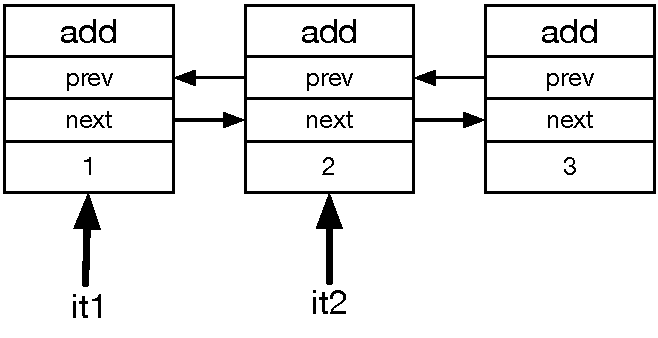
\includegraphics[width=.8\linewidth]{figures/update}
\end{minipage}%
\begin{minipage}{.5\textwidth}
  \centering
  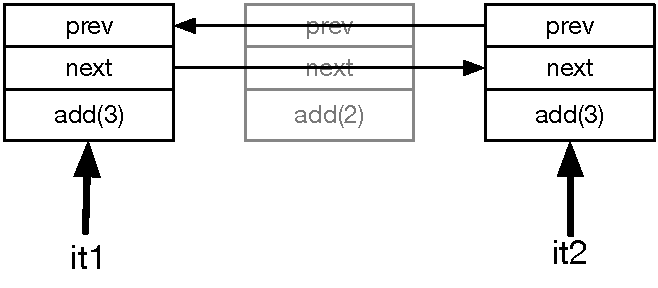
\includegraphics[width=0.8\linewidth]{figures/update2}
\end{minipage}
\begin{minipage}{.5\textwidth}
   \centering
  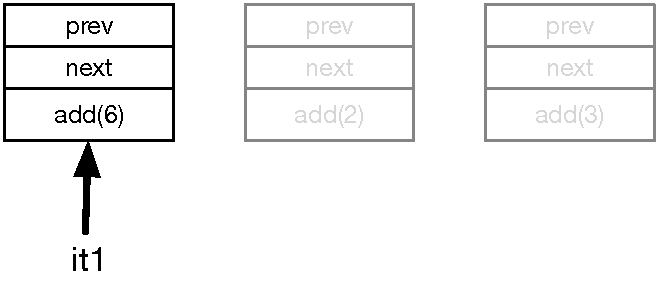
\includegraphics[width=0.8\linewidth]{figures/update3}
\end{minipage}
\caption{Executing the add rule.  }
\label{fig:update_add}
\end{figure}

\subsection{Comprehensions}

Comprehensions were initially presented in the first rule of the SSSP program.

\begin{Verbatim}[fontsize=\scriptsize]
shortest(A, D1, P1), D1 > D2, relax(A, D2, P2)
   -o shortest(A, D2, P2), {B, W | !edge(A, B, W) | relax(B, D2 + W, P2 ++ [B])}.
\end{Verbatim}

The attentive reader will remember that comprehensions are sub-rules, therefore
they should be compiled like normal rules. However, they do not need to return
due to rule priorities since all the combinations of the comprehension must be
derived. However, the rule itself must return if any of its comprehensions has
derived a fact that is used by a higher priority rule.  In the case of the above
example, the rule does not need to return since it has the highest priority and
the \texttt{relax} facts derived in the comprehension are all sent to other
nodes.  The code for the rule is shown below:

\begin{Verbatim}[numbers=left,fontsize=\scriptsize,xleftmargin=\codemargin]
for(auto it1(list("shortest").begin()); it1 != list("shortest").end(); ) {
   fact *f1(*it1);
   for(auto it2(list("relax").begin()); it2 != list("relax").end(); ) {
      fact *f2(*it2);
      if(f1->get_int(1) > f2->get_int(1)) {
         // comprehension code
         for(auto it3(trie("edge").begin()); it3 != trie("edge").end(); ) {
            fact *f3(*it3);
            fact *new_relax(new fact("relax"));
            new_relax->set_int(1, f2->get_int(1) + f3->get_int(2));
            new_relax->set_list(append(f2->get_list(2), list(f3->get_node(1))));
            send_fact(new_relax, f3->get_node(1));
            ++it3;
         }
         f1->set_int(1, f2->get_int(1));
         f1->set_list(2, f2->get_list(2));
         it2 = list("relax").erase(it2);
         goto next;
      }
      ++it2;
   }
   ++it1;
next: continue;
}
\end{Verbatim}

Special care must be taken when the comprehension's sub-rule uses the same
predicates that are derived by the main rule.
Rule inference must be atomic in the sense that after a rule matches, the
comprehensions in the head of the rule can use the facts that were present
before the body of the rule was matched.
Consider a rule with $n$ comprehensions or aggregates, where $CB_i$ and $CH_i$
are the body and head of the comprehension/aggregate, respectively, and $H$
represents the fact templates found in the head of the rule.
The formula used by the compiler to detect conflicts between predicates is the
following:

\[
\bigcup^{n}_i[CB_i \cap H] \cup \bigcup^{n}_i [CB_i \cap \bigcup^{n}_j[CH_j]]
\]

If the result of the formula is not empty, then the compiler disables
optimizations for the conflicting predicates and derives the corresponding facts
into the fact buffer that are then added back into the database.
Fortunately, most rules in LM programs do not show conflicts and thus
can be fully optimized.

\subsection{Aggregates}

Aggregates are similar to comprehensions. They are also sub-rules but a value is
accumulated for each combination of the sub-rule. After all the combinations are
inferred, a final head term is derived with the accumulated term. Consider again
the following PageRank rule:

\begin{Verbatim}[fontsize=\scriptsize]
update(A), pagerank(A, OldRank)
      -o [sum => V | B | neighbor-pagerank(A, B, V) | neighbor-pagerank(A, B, V) |
            pagerank(A, damp/P + (1.0 - damp) * V)].
\end{Verbatim}

The variable \texttt{V} is initialized to \texttt{0.0} and sums all
the PageRank values of the neighbors as seen in the code below. The aggregate
value is then used to update the second argument of the initial
\texttt{pagerank} fact.

\begin{Verbatim}[numbers=left,fontsize=\scriptsize,xleftmargin=\codemargin]
for(auto it1(list("pagerank").begin()); it1 != list("pagerank").end(); ) {
   fact *f1(*it1);
   for(auto it2(list("update").begin()); it2 != list("update").end(); ) {
      fact *f2(*it2);
      double acc(0.0); // aggregate accumulator.
      for(auto it3(list("neighbor-pagerank").begin()); it3 !=
            list("neighbor-pagerank").end(); ) {
         fact *f3(*it3);
         acc += f3->get_float(2);
         ++it3; // the sub-rule has no head since neighbor-pagerank is re-derived
      }
      // head of the aggregate
      f1->set_float(1, damp / P + (1.0 - damp) * V);
      goto next;
   }
   ++it1;
next: continue;
}
\end{Verbatim}
